\documentclass{article}

\usepackage{amsmath}
\usepackage{amsthm}
\usepackage{amsfonts}
\usepackage{thmtools}
\usepackage{stmaryrd}

\usepackage{tikz}

\declaretheorem[numbered=yes,name=Lemma]{lemma}
\declaretheorem[numbered=yes,name=Definition]{definition}

\newcommand{\update}[2]{[#1 \mapsto #2]}%TODO change this to nicer notation \Phi[heap.a \mapsto w]

\newcommand{\var}[1]{\mathit{#1}}
\newcommand{\hv}{hv}
\newcommand{\rv}{rv}
\newcommand{\lv}{lv}
\newcommand{\pc}{\mathit{pc}}
\newcommand{\pcreg}{\mathrm{pc}}
\newcommand{\addr}{a}
\newcommand{\word}{w}
\newcommand{\start}{start}
\newcommand{\addrend}{end}
\newcommand{\mem}{mem}
\newcommand{\reg}{reg}
\newcommand{\heap}{heap}
\newcommand{\mode}{mode}
\newcommand{\perm}{perm}

\newcommand{\failed}{\mathit{failed}}
\newcommand{\halted}{\mathit{halted}}

\newcommand{\false}{\mathit{false}}
\newcommand{\true}{\mathit{true}}

\newcommand{\plainfun}[1]{\mathit{#1}}
\newcommand{\decode}{\plainfun{decode}}
\newcommand{\updatePcPerm}[1]{\plainfun{updatePcPerm}}
\newcommand{\executeAllowed}[1]{\plainfun{executeAllowed}(#1)}
\newcommand{\nonZero}[1]{\plainfun{nonZero}(#1)}
\newcommand{\readAllowed}[1]{\plainfun{readAllowed}(#1)}
\newcommand{\writeAllowed}[1]{\plainfun{writeAllowed}(#1)}

\newcommand{\plaindom}[1]{\mathrm{#1}}
\newcommand{\Caps}{\plaindom{Cap}}
\newcommand{\Words}{\plaindom{Word}}
\newcommand{\Addrs}{\plaindom{Addr}}
\newcommand{\Mems}{\plaindom{Mem}}
\newcommand{\RegName}{\plaindom{RegName}}
\newcommand{\Regs}{\plaindom{Reg}}
\newcommand{\Heaps}{\plaindom{Heap}}
\newcommand{\Confs}{\plaindom{Conf}}
\newcommand{\Instrs}{\plaindom{Instructions}}
\newcommand{\nats}{\mathbb{N}}

\newcommand{\Perms}{\plaindom{Perm}}

\newcommand{\refreg}[1]{\lfloor #1 \rfloor}
\newcommand{\refheap}[1]{\langle #1 \rangle_h}

\newcommand{\instr}[1]{\mathtt{#1}}
\newcommand{\fail}{\instr{fail}}
\newcommand{\halt}{\instr{halt}}
\newcommand{\oneinstr}[2]{\instr{#1} \; #2}
\newcommand{\jmp}[1]{\oneinstr{jmp}{#1}}


\newcommand{\twoinstr}[3]{\instr{#1} \; #2 \; #3}
\newcommand{\jnz}[2]{\twoinstr{jnz}{#1}{#2}}
\newcommand{\isptr}[2]{\twoinstr{isptr}{#1}{#2}}
\newcommand{\setptr}[2]{\twoinstr{setptr}{#1}{#2}}
\newcommand{\move}[2]{\twoinstr{move}{#1}{#2}}
\newcommand{\store}[2]{\twoinstr{store}{#1}{#2}}
\newcommand{\load}[2]{\twoinstr{load}{#1}{#2}}
\newcommand{\lea}[2]{\twoinstr{lea}{#1}{#2}}

\newcommand{\threeinstr}[4]{\instr{#1} \; #2 \; #3 \; #4}
\newcommand{\restrict}[3]{\threeinstr{restrict}{#1}{#2}{#3}}
\newcommand{\subseg}[3]{\threeinstr{subseg}{#1}{#2}{#3}}
\newcommand{\plus}[3]{\threeinstr{plus}{#1}{#2}{#3}}

\newcommand{\plainperm}[1]{\mathrm{#1}}
\newcommand{\readonly}{\plainperm{ro}}
\newcommand{\readwrite}{\plainperm{rw}}
\newcommand{\exec}{\plainperm{rx}}
\newcommand{\entry}{\plainperm{e}}
\newcommand{\rwx}{\plainperm{rwx}}
\newcommand{\noperm}{\plainperm{o}}

\newcommand{\sem}[1]{\left\llbracket #1 \right\rrbracket}

\begin{document}
$\RegName$ contains $\pcreg$, but is otherwise some undefined, finite set.
\begin{align*}
\Addrs &::= \nats & & &
\Words &::= \Caps + \nats \\
\Regs  &::= \RegName \rightarrow \Words & & &
\Heaps &::= \Addrs \rightarrow \Words \\
\Perms &::= \{\readonly, \readwrite, \exec, \entry, \rwx, \noperm \} & & &
\Mems  &::= \Regs \times \Heaps \\
\Caps  &::= \Perms \times \Addrs \times \Addrs \times \Addrs & & &
\Confs &::= \Mems + \{\failed, \halted\}
\end{align*}

\begin{figure}[!h]
  \centering
  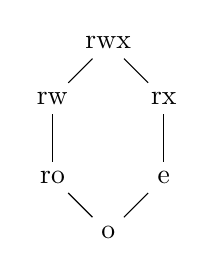
\begin{tikzpicture}[main node/.style={}]
  \node[main node] (1) {$\rwx$};
  \node[main node] (2) [below right of=1] {$\exec$};
  \node[main node] (3) [below of=2] {$\entry$};
  \node[main node] (4) [below left of=1] {$\readwrite$};
  \node[main node] (5) [below of=4] {$\readonly$};
  \node[main node] (6) [below right of=5] {$\noperm$};

  \path[every node/.style={font=\sffamily\small}]
    (1) edge (2)
    (2) edge (3)
    (3) edge (6)
    (1) edge (4)
    (4) edge (5)
    (5) edge (6);
\end{tikzpicture}
\caption{Permission hierarchy}
\label{fig:perm-hier}
\end{figure}
Notation:
$$\begin{array}{rcl}
i       &\in& \Instrs \\
r       &\in& \RegName\\
\mem    &::=& (\reg,\heap)\\
\pc     &\in& \Caps \\
\pcreg  &\in& \RegName \\
\Phi    &::=& \mem \in \Confs\\
\addr   &\in& \Addrs\\
\perm   &\in& \Perms\\
(\perm,\start,\addrend,\addr) &\in& \Caps \\
\end{array}$$
Further definitions:
$$\begin{array}{rcl}
\lv    &::=& \refreg{r} \\
\hv    &::=& \refheap{r}\\
\rv    &::=& n \mid \lv \\
i      &::=& \fail \mid \halt \mid 
             \jmp{\lv} \mid \jnz{\lv}{\rv} \mid
             \isptr{\lv}{\rv} \mid \setptr{\lv}{\rv} \mid \\
       &   & \lea{\lv}{\rv} \mid\move{\lv}{\rv} \mid \load{\lv}{\hv} \mid \store{\hv}{\rv} \mid  \\
       &   & \restrict{\lv}{\rv}{\rv} \mid \subseg{\lv}{\rv}{\rv} \mid \plus{\lv}{\rv}{\rv}
\end{array}$$

\begin{align*}
\decode &:\nats \rightarrow \Instrs
\end{align*}
%TODO for some decode function

\begin{align*}
\Phi & \rightarrow \sem{\decode(\Phi.\reg(\pcreg))}(\Phi) & & \text{if $\Phi.\reg(\pcreg) = (\exec{\_},{\_},{\_})$} \\
\Phi & \rightarrow \failed                                      & & \text{otherwise}
\end{align*}
\begin{align*}
  \executeAllowed{\perm} &=
                           \begin{cases}
                             \true & \text{if } \perm \in \{ \rwx, \exec, \entry \} \\
                             \false & \text{otherwise}
                           \end{cases} \\
  \readAllowed{\perm} &=
                           \begin{cases}
                             \true & \text{if } \perm \in \{ \rwx, \exec, \readwrite, \readonly \} \\
                             \false & \text{otherwise}
                           \end{cases} \\
  \writeAllowed{\perm} &=
                           \begin{cases}
                             \true & \text{if } \perm \in \{ \rwx, \readwrite\} \\
                             \false & \text{otherwise}
                           \end{cases} \\
  \updatePcPerm{\perm,\start,\addrend,\addr} &=
                                     \begin{cases}
                                       (\perm,\start,\addrend,\addr) & \text{if $\perm\in\{ \rwx, \exec \}$} \\
                                       (\exec,\start,\addrend,\addr) & \text{if $\perm = \entry$}
                                     \end{cases} \\
  \nonZero{w} &=
                \begin{cases}
                  \true & \text{if $w\in \Caps$ or $w\in \nats$ and $w \neq 0$}\\
                  \false & \text{otherwise}
                \end{cases}
\end{align*}
%TODO: \Phi.reg(rv) to some other notation. It should only look up reg, if it is a regname otherwise just the litteral.
%TODO: Update semantics according to changes.
\begin{align*}
  \sem{\fail}(\Phi)     & = \failed \\
  \sem{\halt}(\Phi)     & = \halted \\
  \sem{\jmp{\lv}}(\Phi) & = \begin{cases}
                            (\Phi.\reg\update{\pcreg}{\updatePcPerm{c}}) & \text{if }\Phi.reg(lv) = c \\
                                                                         & \text{  and }c=(\perm,\start,addrend,\addr)\\
                                                                         & \text{  and }\executeAllowed{\perm}\\
                            \failed & \text{otherwise }
                            \end{cases} \\
  \sem{\jnz{\lv}{\rv}}(\Phi) & = \begin{cases}
                            \Phi.\reg\update{\pcreg}{\updatePcPerm{\var{c}}} &
                            \begin{array}{l}
                              \text{if $\nonZero{\Phi.\reg(\rv)}$} \\ 
                              \text{  and $\Phi.reg(lv) = c$} \\
                              \text{  and $c=(\perm,\start,\addrend,\addr)$}\\
                              \text{  and $\executeAllowed{\perm}$}
                            \end{array}
                            \\ %TODO Maybe combine with jump. (failed + this)
                            \Phi.\reg\update{\pcreg}{\Phi.\reg(\pcreg) + 1} & \text{if not $\nonZero{\Phi.\reg(\rv)}$}\\
                            \failed & \text{otherwise }
                            \end{cases} \\
 \sem{\load{\refreg{r_1}}{\refheap{r_2}}} & =
                                 \begin{cases}
                                   \Phi.\reg\update{r_1}{\var{w}} &
                                   \begin{array}{l}
                                     \text{if }\Phi.\reg(r_2) = (\perm,\start,\addrend,\addr)\\
                                     \text{  and }\readAllowed{\perm} \text{ and } \var{w} = \Phi.\heap(\addr)
                                   \end{array}\\
                                   \failed & \text{otherwise }
                                 \end{cases}\\
 \sem{\store{\refheap{r_1}}{\refreg{r_2}}} & =
                                 \begin{cases}
                                   \Phi.\heap\update{\addr}{\var{w}} &
                                   \begin{array}{l}
                                     \text{if }\Phi.\reg(r_1) = (\perm,\start,\addrend,\addr)\\
                                     \text{  and }\writeAllowed{\perm} \text{ and } \var{w} = \Phi.\reg(r_2)
                                   \end{array}\\
                                   \failed & \text{otherwise }
                                 \end{cases}\\
 \sem{\move{\refreg{r_1}}{\rv}} & =
                                 \begin{cases}
                                   \Phi.\reg\update{r_1}{\Phi.\reg(\rv)} & \text{if $r_1 \neq \pcreg$} \\
                                   \failed   & \text{otherwise }
                                 \end{cases}\\
\end{align*}


\end{document}
